\hypertarget{_t_com_sample_adaptive_offset_8cpp}{}\section{Lib/\+T\+Lib\+Common/\+T\+Com\+Sample\+Adaptive\+Offset.cpp File Reference}
\label{_t_com_sample_adaptive_offset_8cpp}\index{Lib/\+T\+Lib\+Common/\+T\+Com\+Sample\+Adaptive\+Offset.\+cpp@{Lib/\+T\+Lib\+Common/\+T\+Com\+Sample\+Adaptive\+Offset.\+cpp}}


sample adaptive offset class  


{\ttfamily \#include \char`\"{}T\+Com\+Sample\+Adaptive\+Offset.\+h\char`\"{}}\newline
{\ttfamily \#include $<$string.\+h$>$}\newline
{\ttfamily \#include $<$stdlib.\+h$>$}\newline
{\ttfamily \#include $<$stdio.\+h$>$}\newline
{\ttfamily \#include $<$math.\+h$>$}\newline
Include dependency graph for T\+Com\+Sample\+Adaptive\+Offset.\+cpp\+:
\nopagebreak
\begin{figure}[H]
\begin{center}
\leavevmode
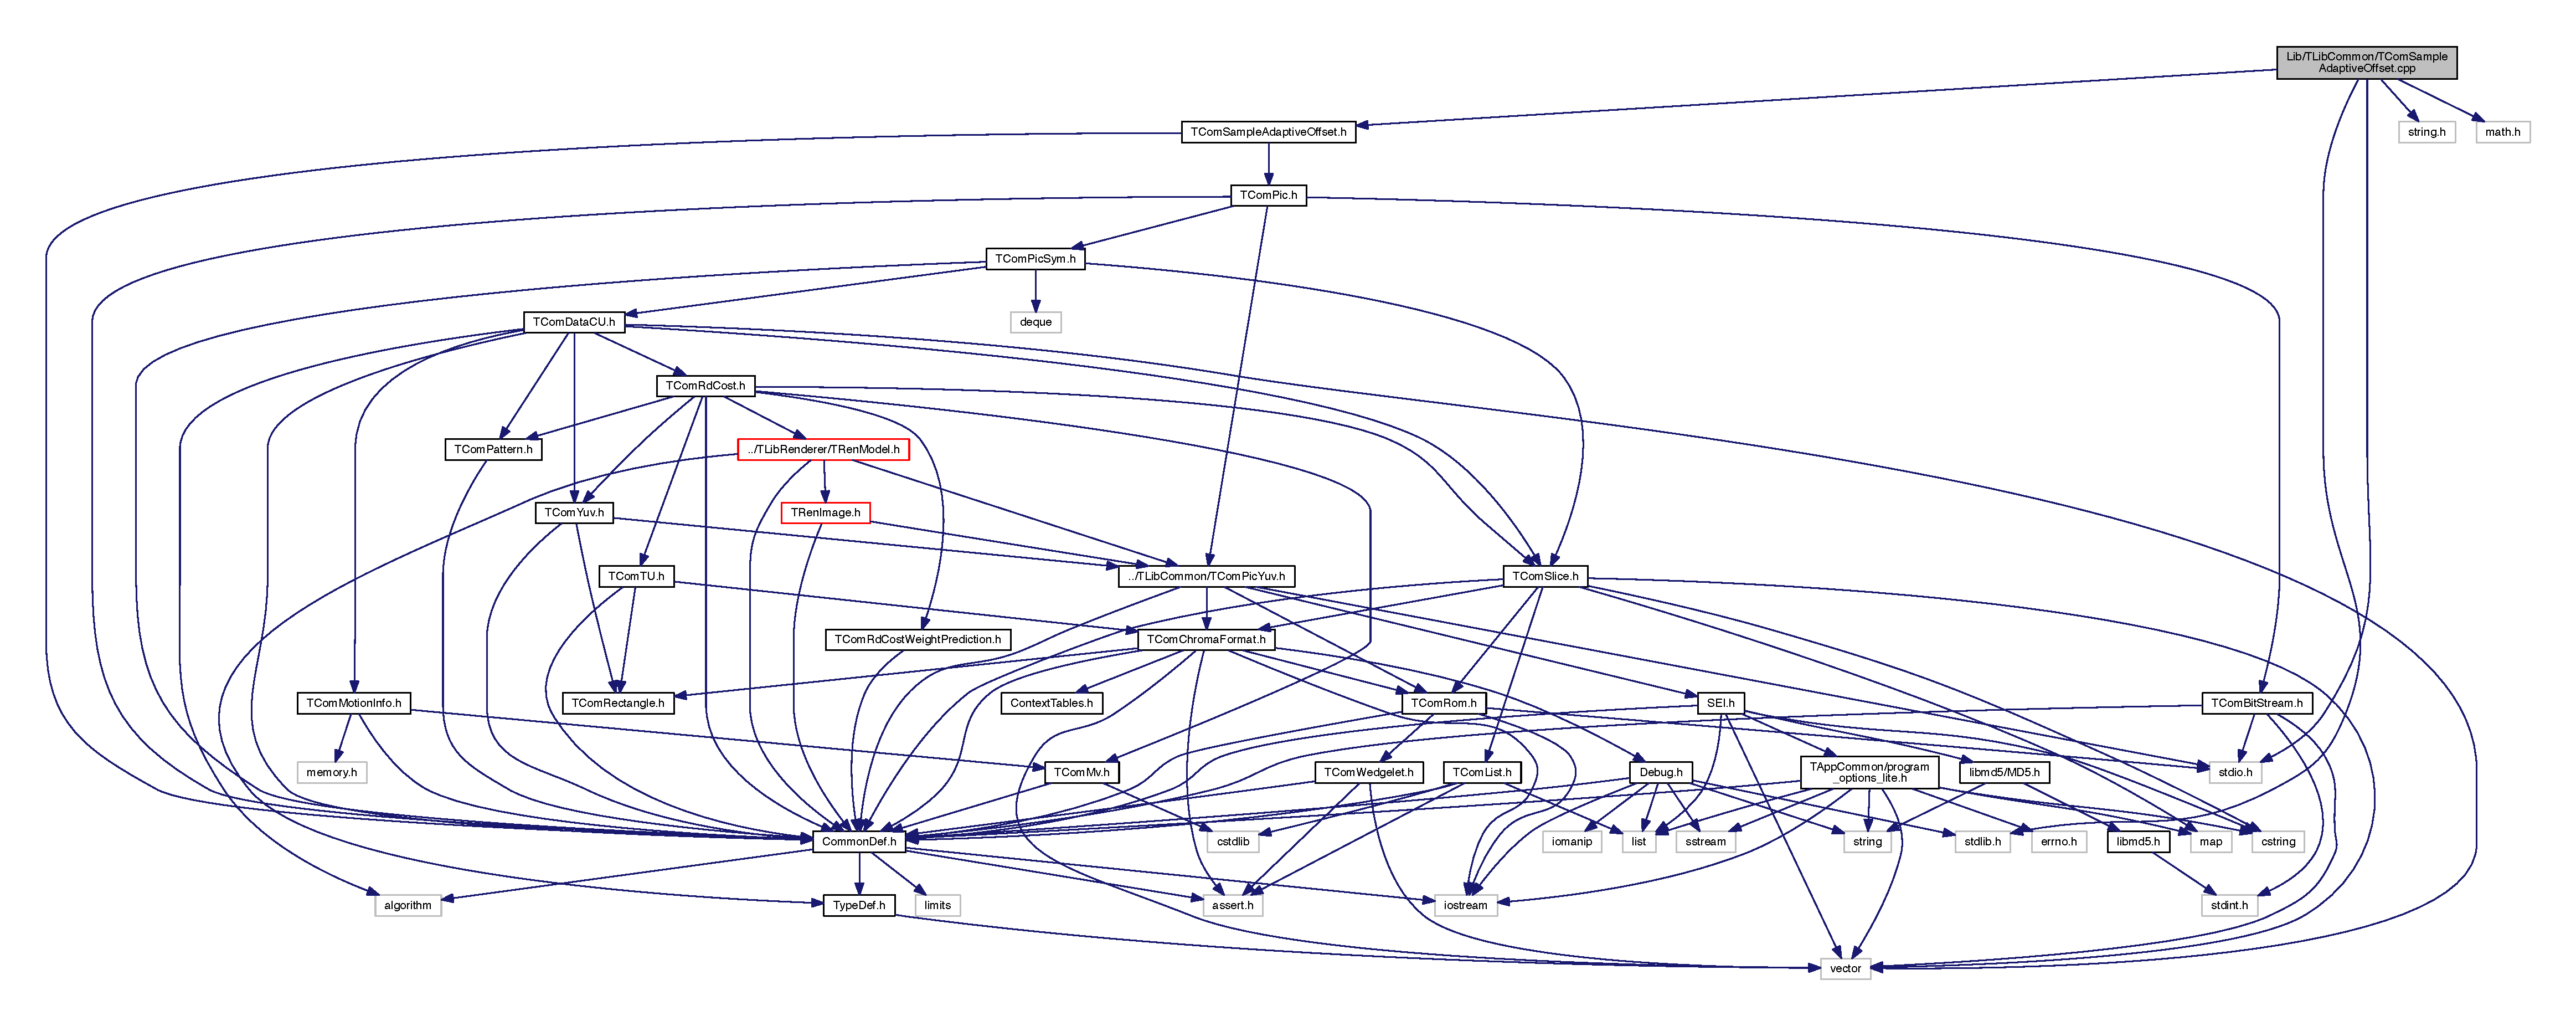
\includegraphics[width=350pt]{da/d4d/_t_com_sample_adaptive_offset_8cpp__incl}
\end{center}
\end{figure}


\subsection{Detailed Description}
sample adaptive offset class 

